The \textit{Notification} module is responsible for keeping the user informed 
as to when the benchmarking on their work is done. this is in place because
results will often not be instant due to factors such as queues because of server
load or algorithm needing a large of time to be throughly benchmarked. Once the
benchmarking is completed, the user will be notified by email that they can now
view their results.

\subsection{Scope}
The scope for the users module is shown in Figure \ref{Notifications Scope}
\begin{figure}[H]
	\begin{center}
		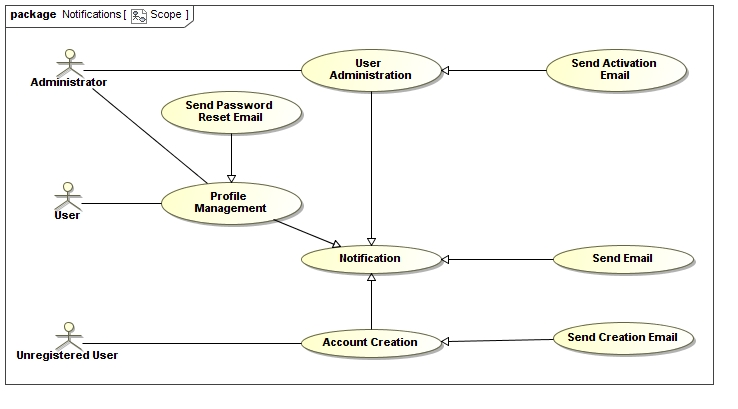
\includegraphics[scale=0.5]{../Diagrams and Charts/Notificatiosn/Scope.jpg}
		\caption{Notifications Scope}
	\end{center}
	\label{Notifications Scope}
\end{figure}
The scope of the Notification module includes:
\begin{itemize}
	\item Alerting the user that their benchmarking is finished
	\item Directing their users to where they can view their results
\end{itemize}

\subsection{Domain Model}
The domain model for the notifications module is shown in Figure \ref{Notifications Domain Model}
\begin{figure}[H]
	\begin{center}
		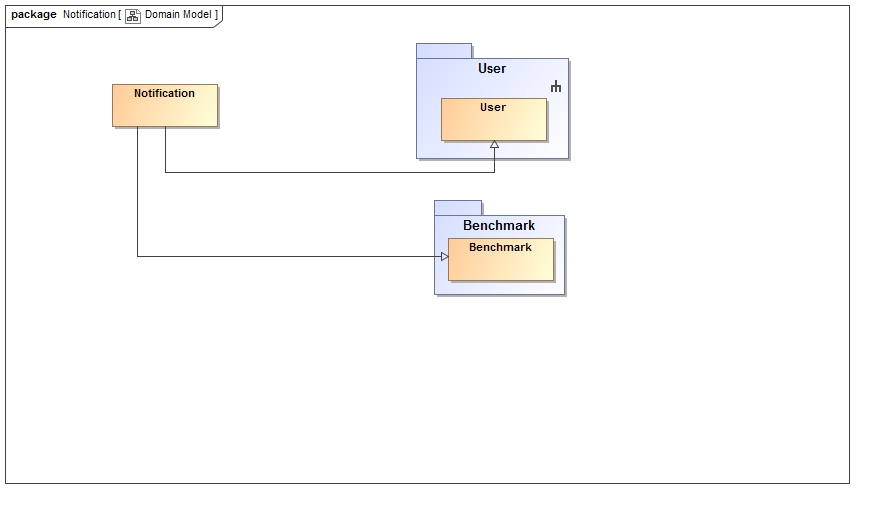
\includegraphics[scale=1.0]{../Diagrams and Charts/Notifications/Domain Model.jpg}  
		\caption{Notifications Domain Model}
	\end{center}
	\label{Notifications Domain Model}
\end{figure}